%(BEGIN_QUESTION)
% Copyright 2006, Tony R. Kuphaldt, released under the Creative Commons Attribution License (v 1.0)
% This means you may do almost anything with this work of mine, so long as you give me proper credit

Bestem hvordan denne bourdonrør-mekanismen i et manometer må justeres for å korrigere kalibreringsfeilen vist i «As-Found»-kalibreringstabellen.

\vskip 10pt

\hbox{ % Encloses both image and table into a horizontal group

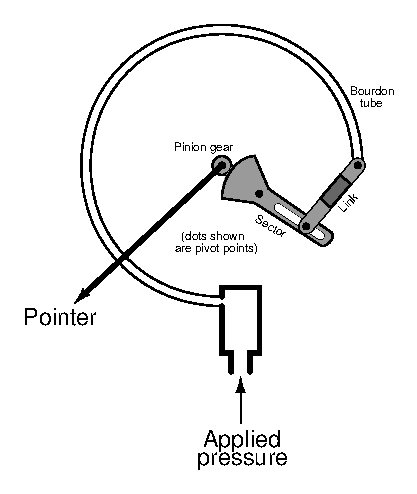
\includegraphics[width=15.5cm]{i00464x01.eps} \hskip 30pt

% No blank lines allowed between lines of an \halign structure!
% I use comments (%) instead, so that TeX doesn't choke.

%$$\vbox{\offinterlineskip
\vbox{\offinterlineskip
\halign{\strut
\vrule \quad\hfil # \ \hfil &
\vrule \quad\hfil # \ \hfil \vrule \cr
\noalign{\hrule}
%
% First row
Påtrykt trykk & Målerindikasjon \cr
%
(PSI) & (PSI) \cr
%
\noalign{\hrule}
%
% Another row
0 & 0 \cr
%
\noalign{\hrule}
%
% Another row
25 & 27.5 \cr
%
\noalign{\hrule}
%
% Another row
50 & 55 \cr
%
\noalign{\hrule}
%
% Another row
75 & 82.5 \cr
%
\noalign{\hrule}
%
% Another row
100 & 110 \cr
%
\noalign{\hrule}
} % End of \halign
} % End of \vbox
%}$$ % End of \vbox

} % End of \hbox enclosing both image and table

\vskip 10pt

Etter inspeksjon av måleren ser du at følgende justeringer er mulige:

\begin{itemize}
\item{} Forlenge «link»-leddet
\item{} Forkorte «link»-leddet
\item{} Flytte leddpunktet mellom «link» og «sector» nærmere pinjonghjulet
\item{} Flytte leddpunktet mellom «link» og «sector» lengre fra pinjonghjulet
\item{} Flytte viseren med klokken på «pinion gear»-akselen
\item{} Flytte viseren mot klokken på «pinion gear»-akselen
\item{} Bøye bourdonrøret oppover (rettere)
\item{} Bøye bourdonrøret nedover (mer bøyd)
\end{itemize}

\vskip 10pt

\noindent
Det gis poeng for å bestemme følgende:

\begin{itemize}
\item{} Identifiser hvilken del av mekanismen som må justeres for å korrigere kalibreringen, og i hvilken retning den må justeres
\vskip 5pt
\item{} Forklar hvorfor denne justeringen fungerer:
\end{itemize}

\underbar{file i00464}
%(END_QUESTION)





%(BEGIN_ANSWER)

\begin{itemize}
\item{} {\bf (5 poeng)} Identifiser hvilken del som skal justeres -- {\bf Flytt leddpunktet mellom «link» og «sector» lengre fra pinjonghjulet}
\vskip 5pt
\item{} {\bf (5 poeng)} Forklar hvorfor dette virker: {\bf Viseren beveger seg for langt i forhold til påtrykt trykk, så vi må redusere mekanismens bevegelsesforsterkning. Ved å flytte «link»-leddet utover (bort fra sektorhjulets pivot), trengs større bevegelse i bourdonrøret for samme viservridning. Med andre ord vil samme bevegelse i bourdonrøret gi mindre viservridning, som er akkurat det vi ønsker.}
\end{itemize}

%(END_ANSWER)





%(BEGIN_NOTES)

{\bf Denne oppgaven er ment for eksamen, ikke arbeidsark!}.

%(END_NOTES)
